\documentclass{ctexart}
\usepackage[table]{xcolor}
\usepackage{template_by_mny}
\usepackage{float} 
\usepackage{listings}
\usepackage[figuresright]{rotating}
\lstset{basicstyle=\ttfamily, breaklines=true, frame=single}

\title{迈克尔逊干涉仪实验报告}
\class{物理 32/物理 31}
\name{冯家琦/周方远}
\id{2023011338/2023011263}

\begin{document}
\maketitle

\begin{abstract}
本报告旨在通过使用迈克尔逊干涉仪(Michelson Interferometer)进行一系列实验,来熟悉干涉仪作为高灵敏度测量仪器的应用。实验内容包括调整干涉仪臂长对干涉图样的影响、观察温度变化对光路的影响、验证干涉仪的双输出特性,并测量激光波长。
\end{abstract}

\section{实验原理}
迈克尔逊干涉仪是一种利用分光束器将激光束分成两束,经过反射后再重新合并产生干涉图样的仪器。其工作原理基于光的干涉现象,即两束相干光(如激光)在相遇时,会因为相位差产生构造性干涉或破坏性干涉,形成明亮或暗色的条纹。

当激光束被分光束器分为两束后,它们分别沿着两个臂传播并反射回来,在分光束器处重新合并。如果两臂的长度差导致光程差为波长的整数倍,则会发生构造性干涉;如果光程差为半波长的奇数倍,则会发生破坏性干涉。干涉图样的变化与两臂之间的光程差直接相关,可以通过以下公式描述:

\[ \Delta s = m \lambda \]
其中,\(\Delta s\) 是两臂之间的光程差,\(m\) 是整数(干涉级次),\(\lambda\) 是激光的波长。

当移动其中一个反射镜时,光程差会改变,导致干涉图样的移动。如果镜子移动了距离 \(\Delta x\),则光程差的变化为 \(2\Delta x\)(因为光需要往返两次),干涉图样上会观察到新的亮或暗条纹。通过计算移动距离和观察到的条纹变化次数,可以测量激光的波长:

\[ \lambda = \frac{2 \Delta x}{N} \]
其中,\(\Delta x\) 是镜子的实际移动距离,\(N\) 是干涉图样上的条纹变化次数。


通过这些原理,迈克尔逊干涉仪不仅可以用于测量波长,还可以用于精确测量长度变化、折射率变化等物理量,是实验物理中非常重要的工具。
\section{实验仪器及安装}
\subsection{实验仪器}
本实验使用的仪器包括:
\begin{itemize}
    \item 迈克尔逊干涉仪套件(EDU-MINT2)
    \item 激光源(CPS532-C2 Laser)
    \item 屏幕
    \item 可调节的镜子
    \item 火柴或打火机
\end{itemize}

\subsection{仪器安装}
根据迈克尔逊干涉仪套件用户手册,首先将四个橡胶脚固定在面包板的底部,然后将激光、分光束器、屏幕和可调节的镜子等组件按照说明书步骤组装并调整至适当位置。

\begin{figure}[H]
    \centering
    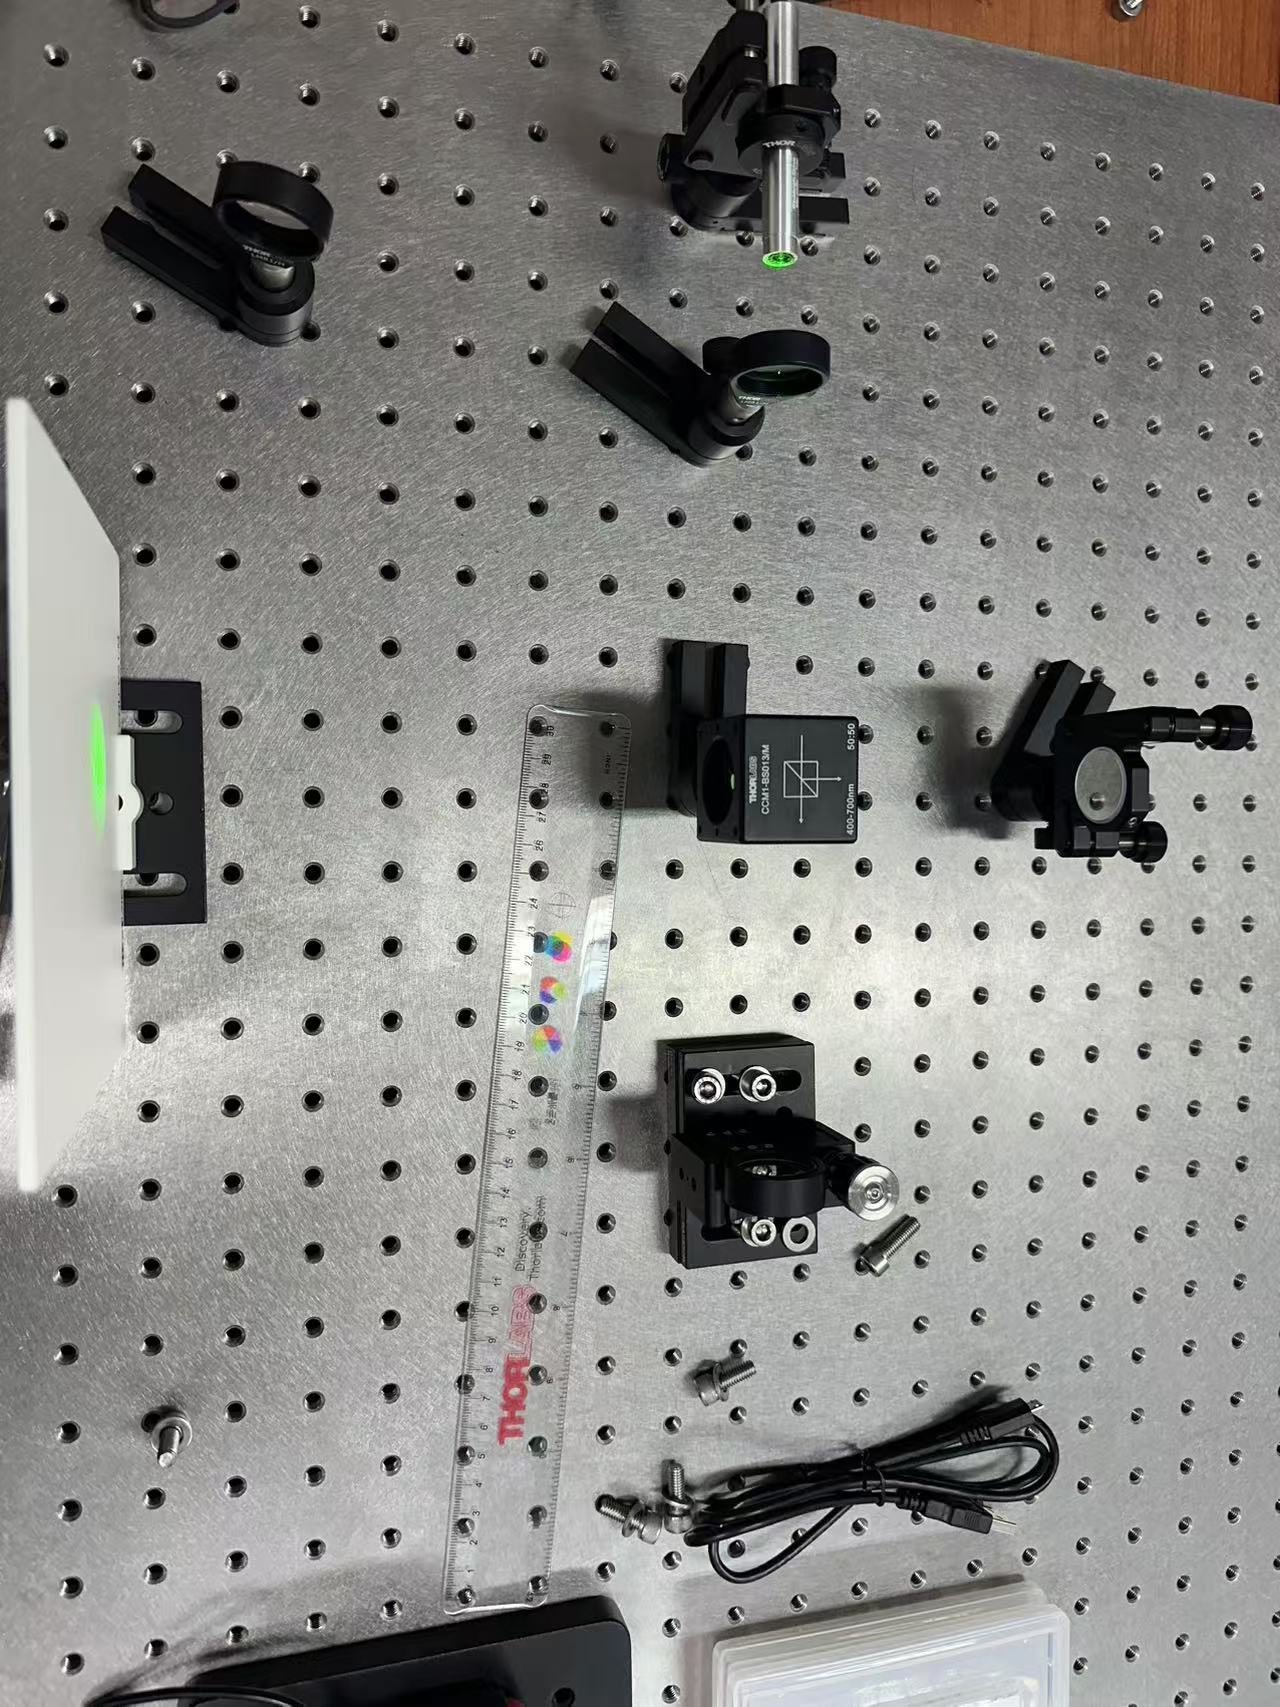
\includegraphics[width=0.4\textwidth]{pictures/微信图片_20241212155934.jpg}
    \caption{光路}
\end{figure}

\section{实验步骤}
\subsection{初步测试}
根据手册中的Exercise 1、3和4,进行以下实验步骤:

\subsubsection{实验1:改变干涉仪臂长对干涉图样的影响}
\begin{enumerate}
    \item 调整迈克尔逊干涉仪,将其中一面镜子移远以改变其中一臂的长度。
    \item 观察干涉图样的变化,与两臂臂长相近时的干涉图样相比较。
    \item 观察到两臂长相差过大时,干涉图样的大小会缩小。
\end{enumerate}

\begin{figure}[H]
    \centering
    \begin{minipage}[b]{0.4\textwidth}
      \centering
      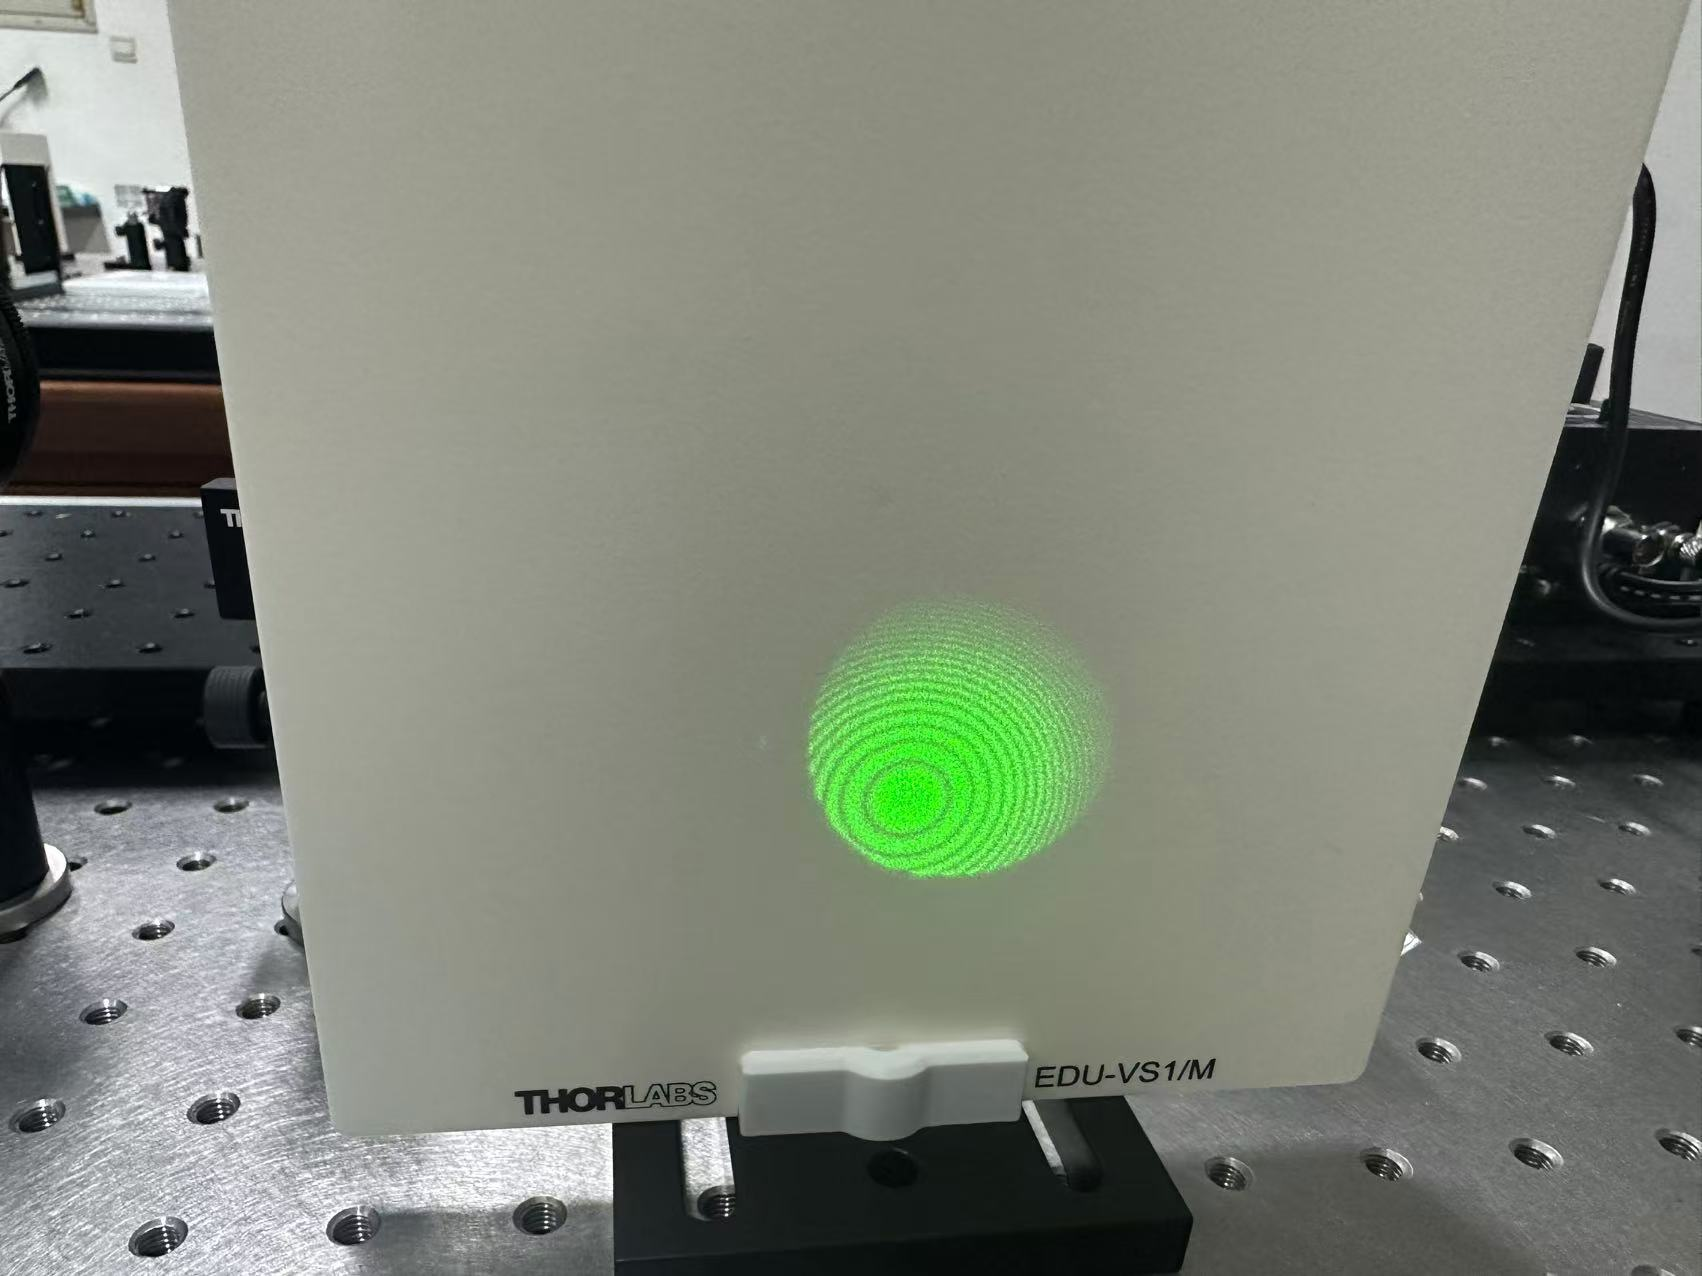
\includegraphics[width=\textwidth]{pictures/微信图片_20241212155855.jpg}
      \caption{两臂等长时的干涉条纹}
    \end{minipage}
    \hspace{0.1\textwidth} % 图片之间的水平间距
    \begin{minipage}[b]{0.4\textwidth}
      \centering
      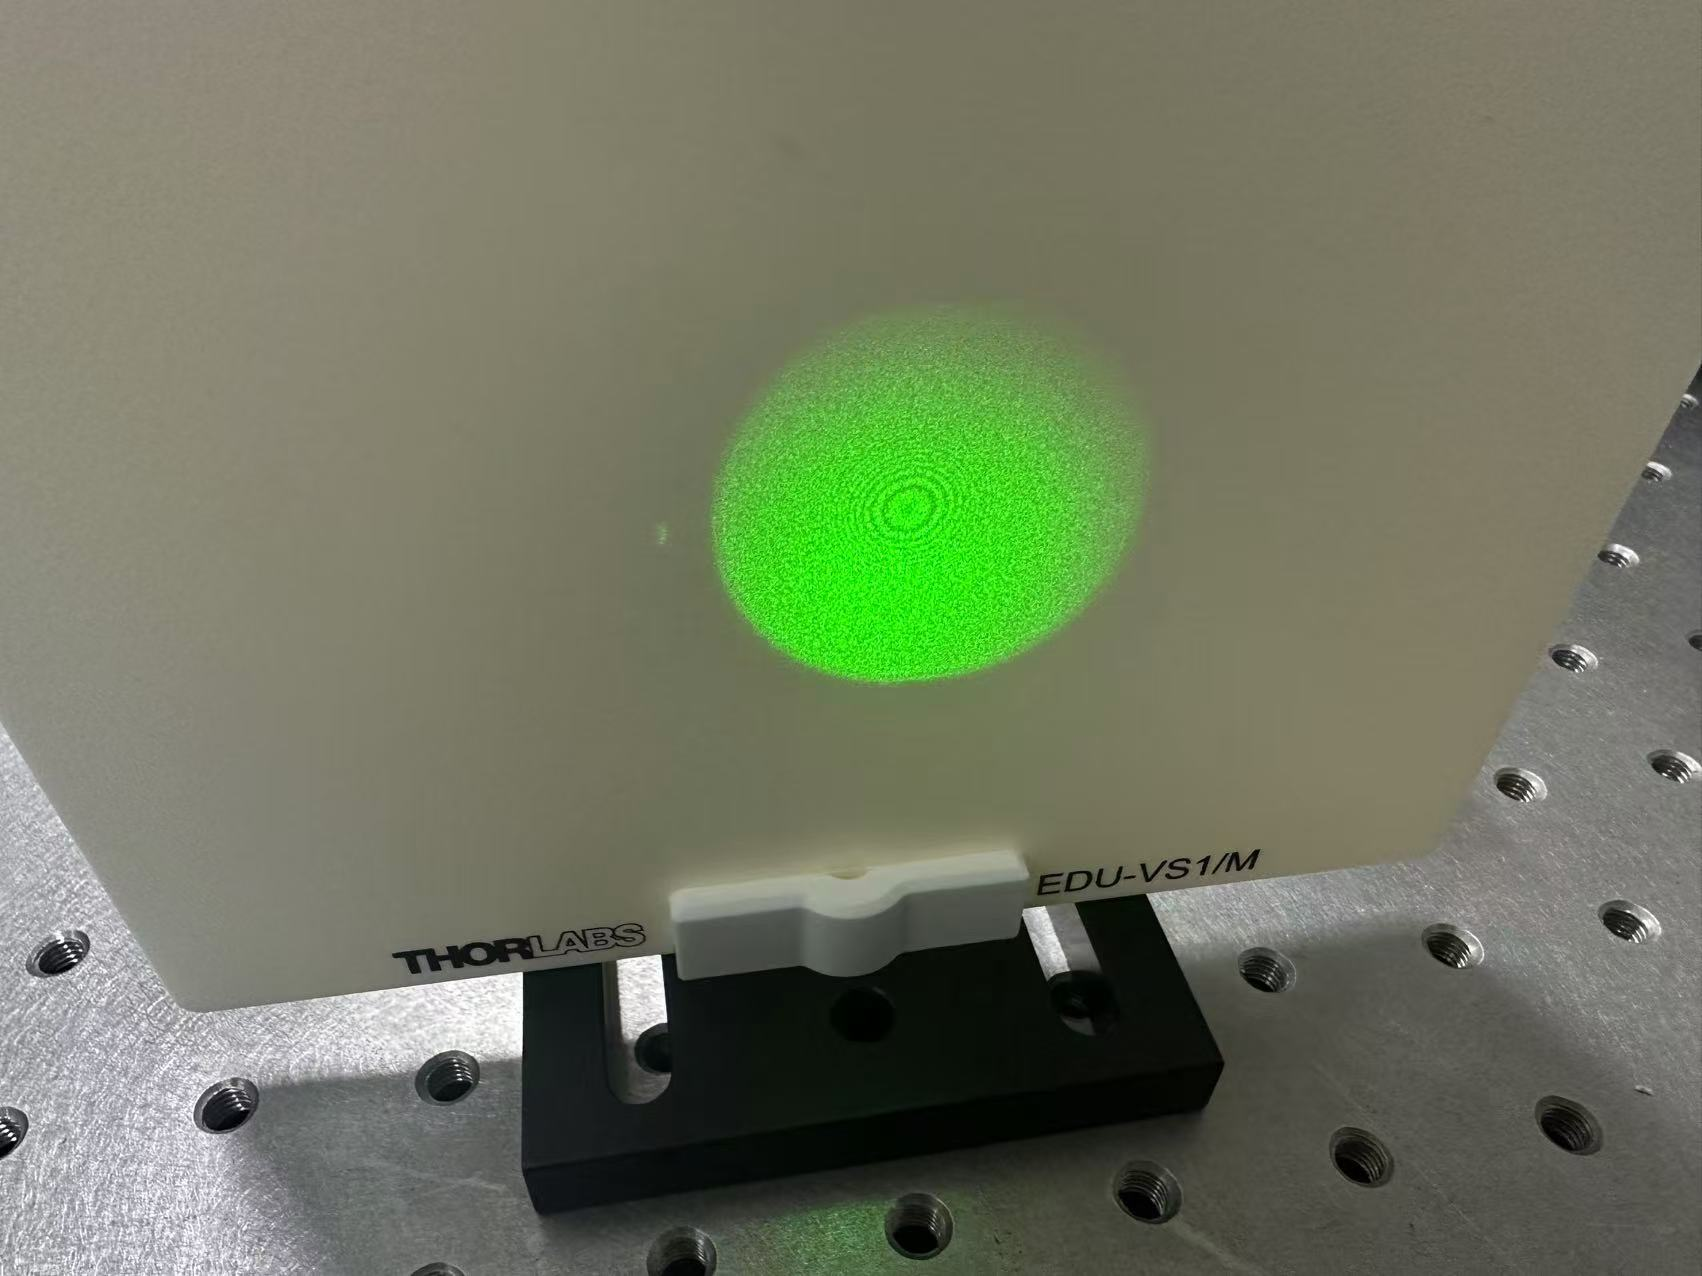
\includegraphics[width=\textwidth]{pictures/微信图片_20241212155927.jpg}
      \caption{两臂不等长时的干涉条纹}
    \end{minipage}
  \end{figure}
\subsubsection{实验3:验证迈克尔逊干涉仪的双输出特性}
\begin{enumerate}
    \item 确保干涉仪已正确组装并调整。
    \item 在分光器和激光器之间再安装一个分光器,将原本分光器输出到激光器一侧的图样输出到屏幕上。
    \item 在屏幕上观察,将原本的干涉图样与射向激光器一侧的输出图样进行比较,记录观察到的差异。
    \item 观察到两个输出图样是互补的关系。
    \item 讨论干涉仪的双输出特性及其对实验结果的影响。
\end{enumerate}

\begin{figure}[H]
    \centering
    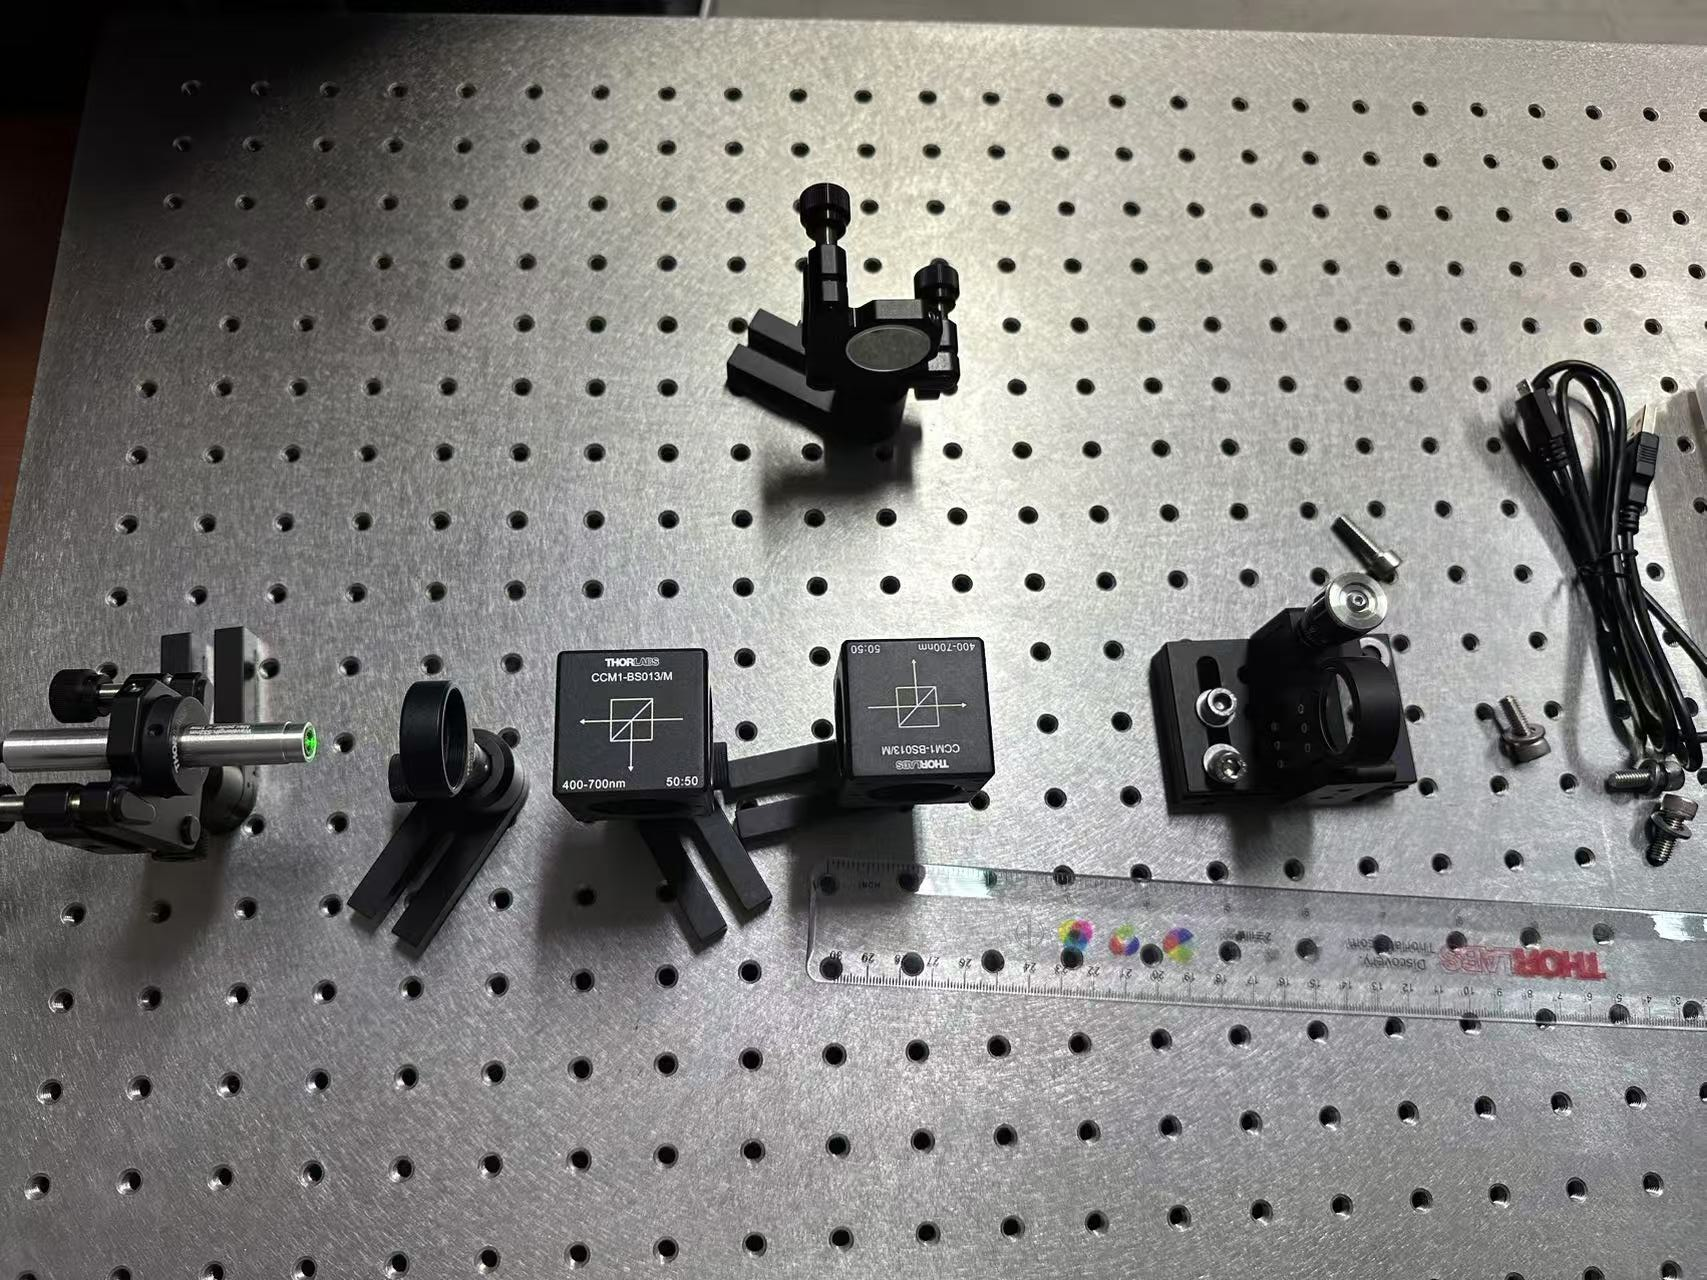
\includegraphics[width=0.4\textwidth]{pictures/微信图片_20241212155941.jpg}
    \caption{光路}
\end{figure}
\begin{figure}[H]
    \centering
    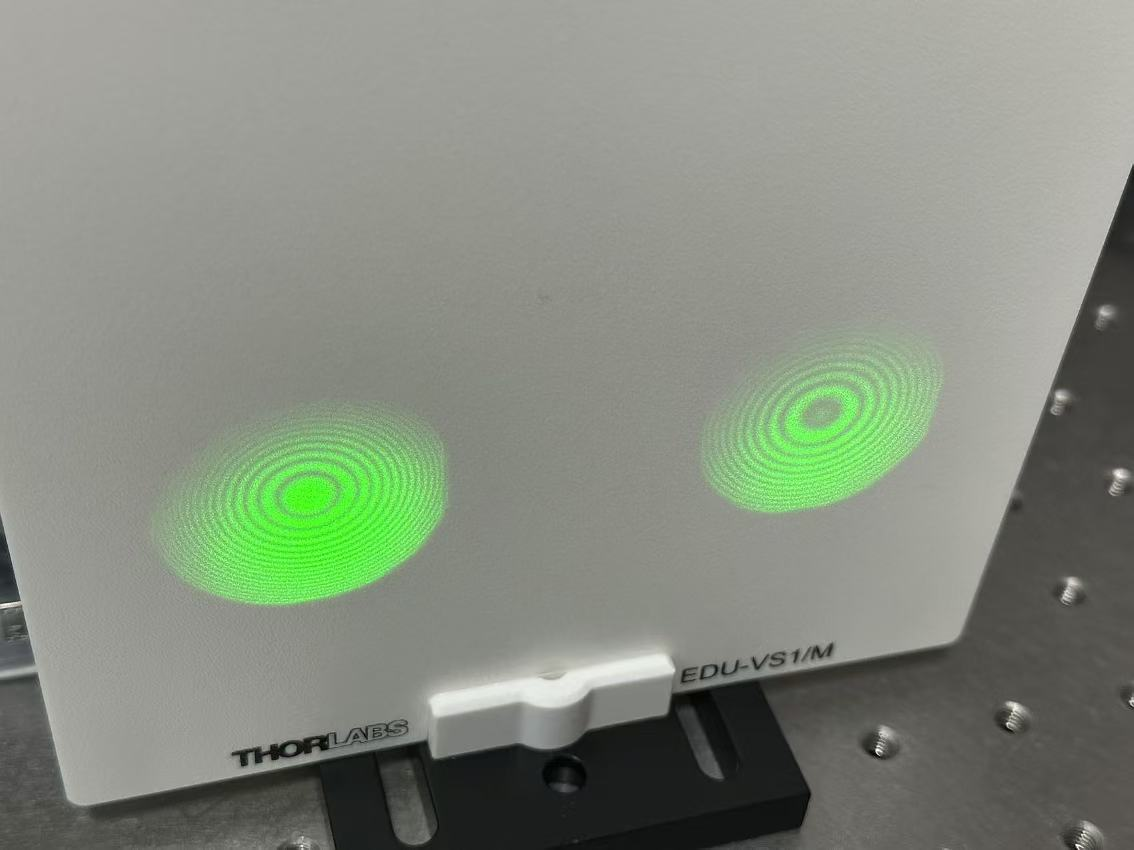
\includegraphics[width=0.4\textwidth]{pictures/微信图片_20241212155938.jpg}
    \caption{双输出图样}
\end{figure}
\subsubsection{实验4:测定激光波长}
\begin{enumerate}
    \item 调整干涉仪,使得干涉图样既不太大也不太小,便于计数光暗变化。
    \item 通过转动微调螺丝改变镜子位置,观察干涉图样的变化。
    \item 记录光暗变化的次数,直到观察到完整的光暗变化周期。
    \item 根据微调螺丝的起始和终止值以及光暗变化的次数,计算激光的波长。公式为:
    \[
    \lambda = \frac{2 \Delta x}{N}
    \]
    其中,\(\Delta x\)为镜子移动的距离,\(N\)为光暗变化的次数。
\end{enumerate}

测量数据及计算结果如下
\begin{table}[H]
    \centering
    \begin{tabular}{|c|c|c|c|}
        \hline
        \rowcolor{yellow!25} 光暗变化的次数 & 镜面位移 [\(\mu m\)] & 计算出的波长 \\
        \hline
        40 & 13.5 & 675 nm  \\
        \hline
        60 & 19.5 & 650 nm  \\
        \hline
        80 & 25 & 625 nm  \\
        \hline
    \end{tabular}
\end{table}

计算得到激光器波长$\lambda=(675+650+625)/3=650 nm$。
\section{实验思考}
\subsection{干涉仪臂长对干涉图样的影响}
如果干涉仪两臂臂长相差过大,则最终聚焦在屏幕上的两个虚拟光源位置就相差过远。此时屏幕上微小的位置变化会导致光程差有较大的变化,因此这时干涉图案就会变小。

\subsection{迈克尔逊干涉仪的双输出特性}
由于迈克尔逊干涉仪的两个输出图样是互补的,因此其中一个图样中光强为零的点对应另一输出中满光强的点。因此,两图样叠加即位满光强的图样,每点的光强在干涉后没有消失只是被分散到两个输出中去了。
\section{总结}
在本实验中,我们通过调整迈克尔逊干涉仪的臂长,成功观察并分析了干涉图样的变化。实验结果表明,干涉图样的变化与臂长调整之间存在直接关系,这与理论预测相符。通过实验,我们不仅加深了对干涉仪工作原理的理解,也提高了实验操作技能。

\end{document}